\section{Results}
  \begin{figure}
  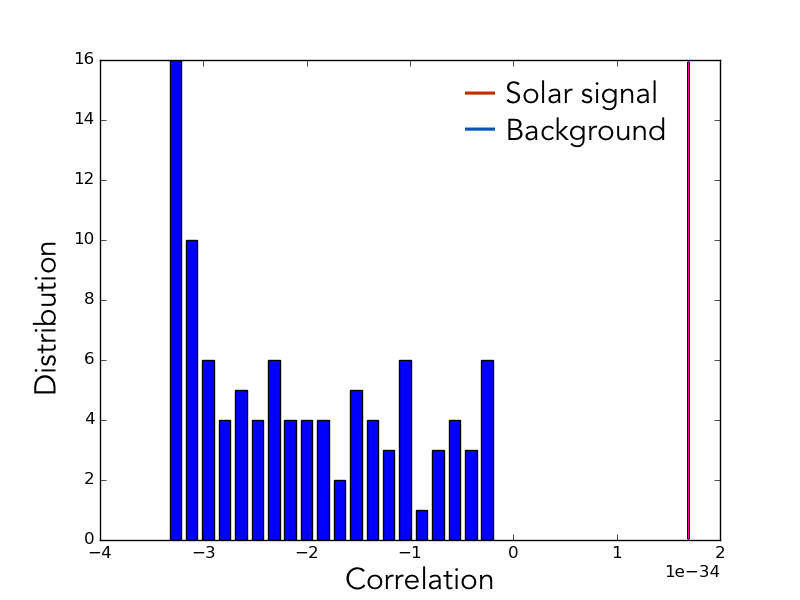
\includegraphics[width=\textwidth]{strain1}
  \caption{Comparison between the Solar signal (single value) and 100 (plotted as a histogram) background data points, summed up over the entire 775.5 hours used from the S6 data (July 2009 - October 2010).}
  \label{strain}
  \end{figure}
To search for a GW signal, the data from the two LIGO detectors was cross-correlated and summed up as follows:
\bigskip \bigskip \bigskip \bigskip \bigskip \bigskip

\begin{equation}
cor = \sum^N h_{L1}(t) \cdot \sum^N h_{H1}(t)
\label{eq:cor}
\end{equation}
where:
\begin{nstabbing}
\phantom{$D_{n40}\ $}\= \kill
N\> is the number of data points: $ \frac { \textrm{the duration}}{\textrm{the time-spacing}},$\\
h\> is the strain signal for H1 and L1 as a function of time.\\
\end{nstabbing}
The duration of the entire data used sums up to 775.5 continuous hours, and the time-spacing is $2.44140625 \times 10^{-4}$ resulting in an N = 3176448. Using equation~\ref{eq:cor}, for both the Solar signal and the background, figure~\ref{strain} was produced with the background plotted as a histogram and the Solar signal represented by the red, vertical line. It can be seen from the plot that the signal from the Sun is indeed higher than the background, with potential for GWs to be detected. The background can be seen to be biased towards negative values. Without further tests and checks, however, no GW detection claim can be made. This result was found towards the end of the project and we plan to continue testing it further soon. 


Using these results, an upper limit on GWs emitted from the Sun in the frequency range of 100 to 300 Hz can be estimated as follows:
\begin{eqnarray}
\label{uplim}
h_{max} & = \sqrt{\frac{ \sum^N h_{L1}(t) \cdot \sum^N h_{H1}(t)}{N}} \\[10pt] \nonumber
& = \sqrt{\frac{ N^2 \, (h_{L1}(t) \cdot  h_{H1}(t))}{N}} \\[10pt] \nonumber
& = \sqrt{ N \, (h_{L1}(t) \cdot  h_{H1}(t))} \nonumber
\end{eqnarray}

Following equation~\ref{uplim} we find that, in this case, the upper limit is $1.215 \times 10^{22}$.
This estimation of the upper limit ignores the noise in the detectors, and a more rigorous estimation can be made (see upper limit estimations in e.g.~\cite{bh1} and~\cite{bh2}).